\documentclass[a4paper, 12pt]{article} %tipo de documento e opções gerais
\usepackage[utf8]{inputenc} %codificação
\usepackage[T1]{fontenc} %codificação
\usepackage[brazil]{babel} %idioma
\usepackage{amsmath,amssymb,amsfonts,amsthm} %padrões em formato matemático
\usepackage[a4paper,top=3cm,bottom=2cm,left=3cm, right=2cm]{geometry} %margens
\usepackage{indentfirst} %primeiro parágrafo com margem
\usepackage{float} %fixar imagens e tabelas
\usepackage{multicol} %várias colunas
\usepackage{multirow} %várias linhas
\usepackage{graphicx} %colocar imagens 
\usepackage{anyfontsize} %qualquer tamanho de letra
\usepackage{setspace} %espaçamento
\usepackage[titles]{tocloft} %padrões de sumário
\usepackage{fontspec} %outros tipos de fonte
\usepackage{fancyhdr} %padronizar o formato do Header
\usepackage[resetlabels,labeled]{multibib} %bibliografia
\usepackage{newfloat} %alterar nome do quadro
\usepackage{csquotes} %adicionar categoria de citações
\usepackage[dvipsnames]{xcolor} %colorir textos
\usepackage[normalem]{ulem} %cortar textos
\usepackage[titles]{tocloft}
\usepackage{afterpage}
\usepackage[T1]{fontenc}
\usepackage{tgbonum}
\usepackage{times}


\newcommand\myemptypage{
    \null
    \thispagestyle{empty}
    \addtocounter{page}{+1}
    \newpage
    }

\makeatletter
\def\ps@Padrao{
    \def\@oddfoot{\null\hfill\thepage}
    \def\@evenfoot{\thepage}%
    \def\@evenhead{\null\hfil\slshape\leftmark }%
    \def\@oddhead{{\slshape\rightmark\hfill }}} %cabeçalho
\makeatother

\pagestyle{Padrao}

\setmainfont{Times New Roman} %fonte arial
\setstretch{1.5} %espaçamento

% ALTERANDO O TÍTULO DAS TABELAS E FIGURAS
\addto\captionsenglish{%
  \renewcommand\tablename{Tabela}
  \renewcommand\figurename{Figura}
}
\DeclareFloatingEnvironment[listname=loq, listname={Lista de Quadros}]{quadro}

% ALTERANDO O SUMÁRIO
\makeatletter
\renewcommand\tableofcontents{
  \null\hfill\textbf{\Large\contentsname}\hfill\null\par
  \@mkboth{\MakeUppercase\contentsname}{\MakeUppercase\contentsname}%
  \@starttoc{toc}}
\makeatother	
\addto\captionsenglish{
  \renewcommand{\contentsname}{Sumário}
  }	

\begin{document}



\begin{titlepage}
\center

\begin{figure}[H]
\cantering
\center

\includegraphics[scale=1]{figuras/unb1.jpg}
\end{figure}
\large
Instituto de Exatas\\
Departamento de Estatística\\

\vspace{3cm}

{\fontsize{16}{18}\selectfont Desigualdades Educacionais no Brasil
}\\[0.4cm]

\vspace{3cm}

Davi Dantas Erthal (20/0016741)

Lucas Castro Linhares Curi (19/0043466)

Maxsuell Nina da Silva (21/1029129)




\vspace{3cm}




Brasília\\
2022

\vfill
\end{titlepage}

%%%%%%%%%%%%%%%%%%%%%%%%%%
%%%%%%%%%%%%%%%%%%%%%%%%%% Modelo de contracapa
%%%%%%%%%%%%%%%%%%%%%%%%%% Se necessário (acho que não)
%%%%%%%%%%%%%%%%%%%%%%%%%%
%%%%%%%%%%%%%%%%%%%%%%%%%%

%%%\begin{titlepage}
%\center
%Davi Dantas Erthal
%\vspace{7cm}

%{\fontsize{16}{18}\selectfont Atividade 3.2 - Teste de Aderência
%}\\[0.4cm]
%\vspace{3cm} 

%\begin{flushright}
%\begin{minipage}{6cm} 
% \parbox[t]{8cm}{\\ 
%Testes
%} \\ \\

%\end{minipage}
%\end{flushright}

%Universidade de Brasília - UNB

%\vspace{5cm}

%\large
%Brasília, 

%\vfill
%\end{titlepage}
%%%%%%%%%%%%%%%%%%%%%%%%%%
%%%%%%%%%%%%%%%%%%%%%%%%%%
%%%%%%%%%%%%%%%%%%%%%%%%%% 
%%%%%%%%%%%%%%%%%%%%%%%%%%
%%%%%%%%%%%%%%%%%%%%%%%%%%




\newpage

\begin{abstract}
    A desigualdade educacional brasileira tem reflexo no ensino e aprendizado da Matemática. De acordo com a neurociência, a educação aos alunos em relação a matemática tem vários fatores externos. Por isso, é importante entender quais fatores podem afetar os resultados nessa disciplina. Utilizando os dados do SAEB para o 5º ano do ensino fundamental no ano de 2017, esse trabalho se propõe a analisar os impactos no resultados das notas em Matemática dos alunos, bem como o tempo gasto com telas. Encontramos que variáveis como Área de localização da escola e frequência à biblioteca afetam significativamente esse resultado. Esse é um estudo exploratório e inferencial, por isso outros estudos sobre o assunto são necessários, afim de aprofundar a analis mais profunda essas relações
\end{abstract}
\tableofcontents
\thispagestyle{empty}

\newpage

\section{Introdução}

O conhecimento da História da Matemática é muito importante para a aprendizagem. Acredita-se que o conhecimento dos fatos históricos pode contribuir para o desenvolvimento do senso crítico dos educandos, pois através de discussões sobre o contexto em que as teorias foram desenvolvidas, poderão estabelecer conexões e com isso compreender de forma mais ampla como se dá a construção do conhecimento. 

É possível também, através desse estudo, que os alunos possam compreender que mesmo os maiores matemáticos da história também tinham dificuldades e passavam por várias privações. No entanto, essas dificuldades não os impediram de desenvolverem capítulos importantes da evolução da Matemática e consequentemente contribuíram decisivamente para o progresso da sociedade e da tecnologia. Sabemos que esse tipo de ensino não é a grande realidade do ensino fundamental na grande maioria. 

Em uma palestra de neurociência e matemática no evento ACAMPS PARTY, uma professora de matemática disse que a maior dificuldade dos alunos em relação a matemática, principalmente nos dias atuais, é que estudar matemática te deixa refém a erros, e as pessoas em sua grande maioria não foram educadas pra resolver problemas e nem gostam de errar. 

O objetivo deste estudo que foi feito é identificar a relação entre o desempenho em matemática e indicadores de desigualdade educacional em termos de sexo, Acesso a biblioteca, tempo de acesso a televisão, computador e vídeo dos estudantes do 5° ano do Ensino Fundamental avaliados pelo SAEB em 2017. Esse tipo de trabalho é fundamental, uma vez que se trata de uma pesquisa que fornece informações importantes para futuras políticas públicas, sobretudo, na área da educação.

\section{Metodologia}
Os dados utilizados foram retirados do Sistema de Avaliação da Educação Básica (SAEB). Trata-se de uma pesquisa realizada pelo INEP para avaliar e aprimorar a qualidade da educação ofertada no Brasil. A amostra utilizada neste trabalho tem como unidade de análise os estudantes do 5° ano do Ensino Fundamental e corresponde ao ano de 2017.

Como o objetivo principal desse estudo é inferir a dificuldade do aprendizado no estudo da matéria matemática, foram escolhidas variáveis que possam ter relação com o desempenho dos alunos nesse aprendizado. Dessa forma, selecionamos como variáveis explicativas Área, Sexo, Acesso à Biblioteca e se possui computador. As variáveis a serem estudadas escolhidas foram a nota em matemática e o tempo de uso de telas.

Para fazer uma análise mais direta, comparamos a nota em Matemática à Área da escola e ao uso de biblioteca/sala de estudo, bem como o tempo de uso de telas com sexo e quantidade de computadores a que o aluno possui acesso. Essa relação é avaliada a partir de gráficos e testes de hipóteses para confirmar se existe significância estatística nessas relações. Dentre os testes utilizados, estão Mann-Whitney, Kruskal-Wallis e o Teste Qui-Quadrado.

\section{Resultados}

Inicialmente, analisamos as variáveis qualitativas de acordo com as suas distribuições de frequência. É possível observar na Tabela \ref{tab1} que existem mais alunos do interior (81,5\%) e quase 50\% deles não possuem computador. A distribuição em relação ao sexo é mais equilibrada, com 51,0\% de meninos e 49\% de meninas compondo a amostra. Entre os que sempre ou quase sempre vão à biblioteca e os que vão de vez em quando somam-se 75,3\%.

\begin{table}[!ht]
\caption{Distribuição de frequências das variáveis qualitativas selecionadas - SAEB, 2017}
\label{tab1}
\centering
\begin{tabular}{l|rr}
\hline
\multicolumn{1}{c|}{\textbf{Características}} & \multicolumn{1}{c}{\textbf{Frequência}} & \multicolumn{1}{c}{\textbf{Frequência Relativa}} \\ \hline
\textbf{Área} &  &  \\
Interior & 1629 & 81,5\% \\
Capital & 371 & 18,5\% \\
 &  &  \\
\textbf{Sexo} &  &  \\
Masculino & 1020 & 51,0\% \\
Feminino & 980 & 49,0\% \\
 &  &  \\
\textbf{Tem Computador?} &  &  \\
Não tem computador & 956 & 47,8\% \\
Sim, 1 & 746 & 37,3\% \\
Sim, 2 & 191 & 9,6\% \\
Sim, 3 & 48 & 2,4\% \\
Sim, 4 ou mais & 26 & 1,3\% \\
Não informado & 23 & 1,2\% \\
 &  &  \\
\textbf{Uso da Biblioteca} &  &  \\
Sempre ou quase sempre & 689 & 34,4\% \\
De vez em quando & 818 & 40,9\% \\
Nunca ou quase nunca & 493 & 24,7\% \\
A escola não possui Biblioteca ou sala de leitura & 0 & 0,0\% \\ \hline
\end{tabular}
\\ \footnotemark{Fonte:Inep (Instituto Nacional de Estudos e Pesquisas Educacionais Anísio Teixeira). }
\end{table}

Enquanto isso, na Tabela \ref{tab2}, notamos que mais de 50\% dos estudantes da amostra passam até duas horas usando alguma tela.

\begin{table}[!ht]
\caption{Distribuição de frequências do tempo de uso de telas - SAEB, 2017}
\label{tab2}
\centering
\begin{tabular}{l|rr}
\hline
\multicolumn{1}{c|}{\textbf{Tempo de Uso de Telas}} & \multicolumn{1}{c}{\textbf{Frequência}} & \multicolumn{1}{c}{\textbf{Frequência Relativa}} \\ \hline
Menos de 1 hora & 608 & 30,4\% \\
Entre 1 e 2 horas & 447 & 22,4\% \\
Mais de 2 horas até 3 & 239 & 12,0\% \\
Mais de 3 horas & 527 & 26,4\% \\
Não vejo TV/Navego na internet/Jogo jogos eletrônicos & 135 & 6,8\% \\
Não informado & 44 & 2,2\% \\ \hline
\end{tabular}
\\ \footnotemark{Fonte:Inep (Instituto Nacional de Estudos e Pesquisas Educacionais Anísio Teixeira). }
\end{table}

Já no Gráfico \ref{fig1}, vemos que a distribuição das notas em Matemática dos alunos tem comportamento que desvia levemente à normal, com caudas um pouco alongadas. Analisando métricas relacionadas, temos que a média das notas foi de 222,1, enquanto a mediana foi de 220.4. O desvio-padrão foi de 46,84. Com isso, calculamos que o Coeficiente de Variação (CV) das notas em Matemática na amostra foi de 21,1\% -- apontando que há uma variabilidade considerável dos dados. A curtose em 2,55 indica que a curva tem leve tendência a ser platocúrtica, enquanto a assimetria, calculada em 0,14, aponta que há uma baixa assimetria positiva. 

\begin{figure}[!ht]
\vspace{-0.25cm}
\caption{Distribuição da nota em Matemática - SAEB, 2017}
\centering
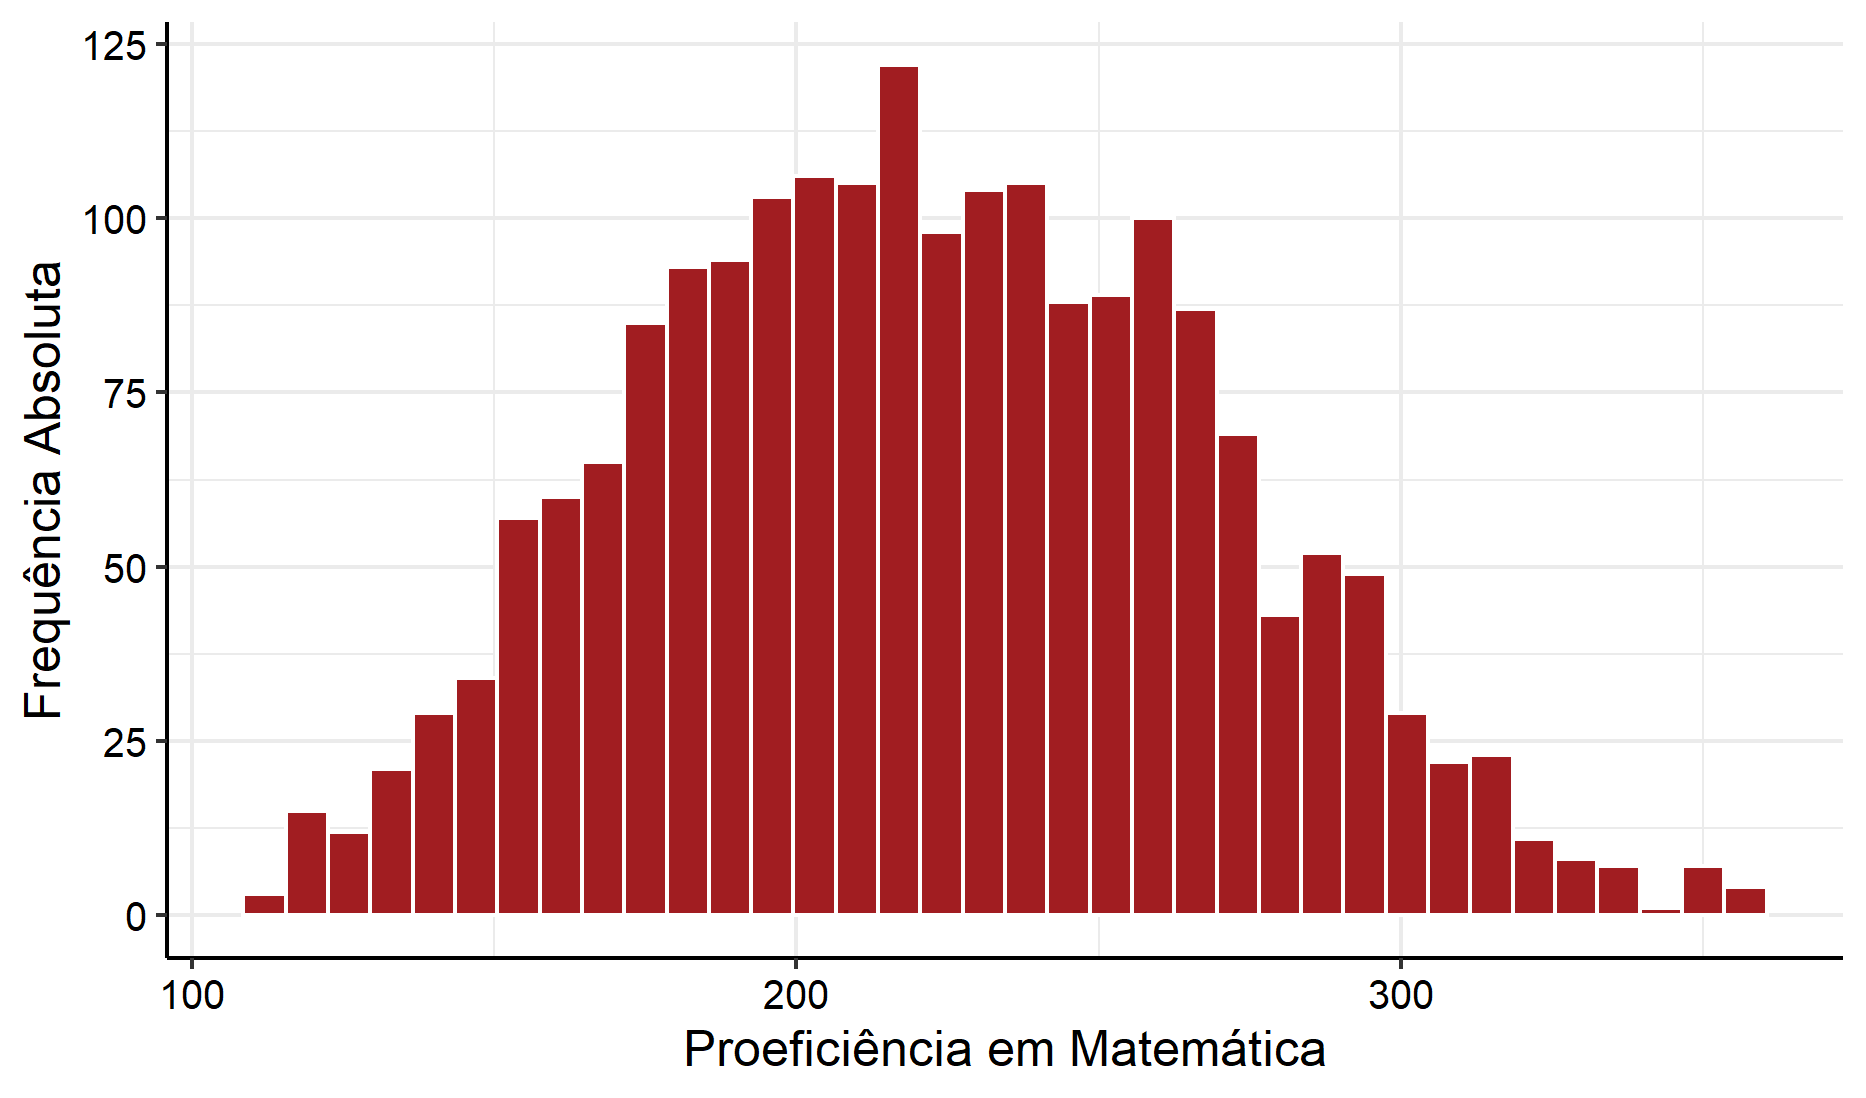
\includegraphics[height=8.2cm,width=12.7cm]{figuras/GRAFICO-NOTAMT-1.png}
\vspace{-0.2cm}
\label{fig1}
\\ \footnotemark{Fonte:Inep (Instituto Nacional de Estudos e Pesquisas Educacionais Anísio Teixeira). }
\end{figure}

Tanto os testes de Shapiro-Wilk quanto Anderson-Darling rejeitam a hipótese nula de normalidade, com p-valor $< 0,01$. No entanto, a amostra não apresenta valores extremos. Isso que leva ao entendimento de que o tamanho da amostra pode estar influenciando no teste.

Afim de avaliar o impacto das variáveis qualitativas em relação à nota de matemática e ao tempo de uso de telas, foram produzidos gráficos para analisar o comportamento das variáveis de interesse em relação às outras variáveis selecionadas. 

No Gráfico \ref{fig2}, temos os boxplots da nota em Matemática segundo a Área de localização da escola. É possível notar que existe diferença na distribuição das categorias. Ainda que os alunos que estudam na capital sejam uma parte menor da amostra (18,5\%), suas notas são maiores do que as dos alunos do interior. Por exemplo, a mediana das notas de alunos da capital é 229.2 enquanto os alunos do interior é 219.3. 

Uma vez que verificamos um desvio na normalidade da variável de nota, realizamos o teste não-paramétrico de Mann-Whitney, considerando que temos duas categorias na variável qualitativa. Nesse caso, obtemos um p-valor $=0.005994$, e com isso temos evidências estatísticas para rejeitar a hipótese nula, um nível de confiança de 99\%. Assim, existe diferença estatística nas notas em matemática dos alunos do interior e da capital.

\begin{figure}[!ht]
\vspace{-0.25cm}
\caption{Distribuição da nota em Matemática segundo Área - SAEB, 2017}
\centering
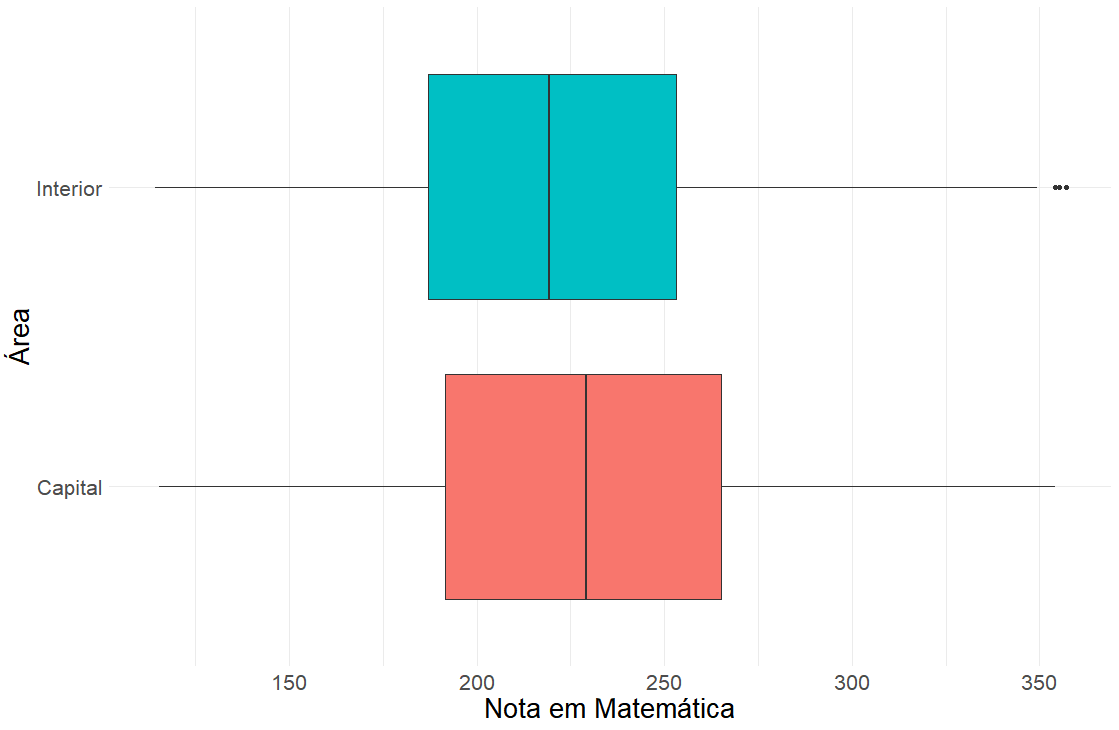
\includegraphics[height=8.2cm,width=12.7cm]{figuras/boxplot_nota_area.png}
\vspace{-0.2cm}
\label{fig2}
\\ \footnotemark{Fonte:Inep (Instituto Nacional de Estudos e Pesquisas Educacionais Anísio Teixeira). }
\end{figure}

No Gráfico \ref{fig3}, comparamos a nota em Matemática em relação ao uso da biblioteca/sala de leitura. Notamos que os alunos que dizem ir sempre ou quase sempre à biblioteca tem uma distribuição com notas menores do que as das outras categorias, com alguns \textit{outliers}. Os alunos que tem maior destaque são aqueles que declararam ir de vez em quando. 

Para confirmar se há diferença, conduzimos o teste de Kruskal-Wallis. Obtemos um p-valor $< 0.01$, o que nos dá evidências estatísticas para rejeitar a hipótese de que não há diferença entre os grupos. Por isso, podemos afirmar que existe divergência nas notas dos alunos com diferentes declarações de frequência à biblioteca/sala de leitura.

\begin{figure}[!ht]
\vspace{-0.25cm}
\caption{Distribuição da nota em Matemática segundo Uso da biblioteca/sala de leitura - SAEB, 2017}
\centering
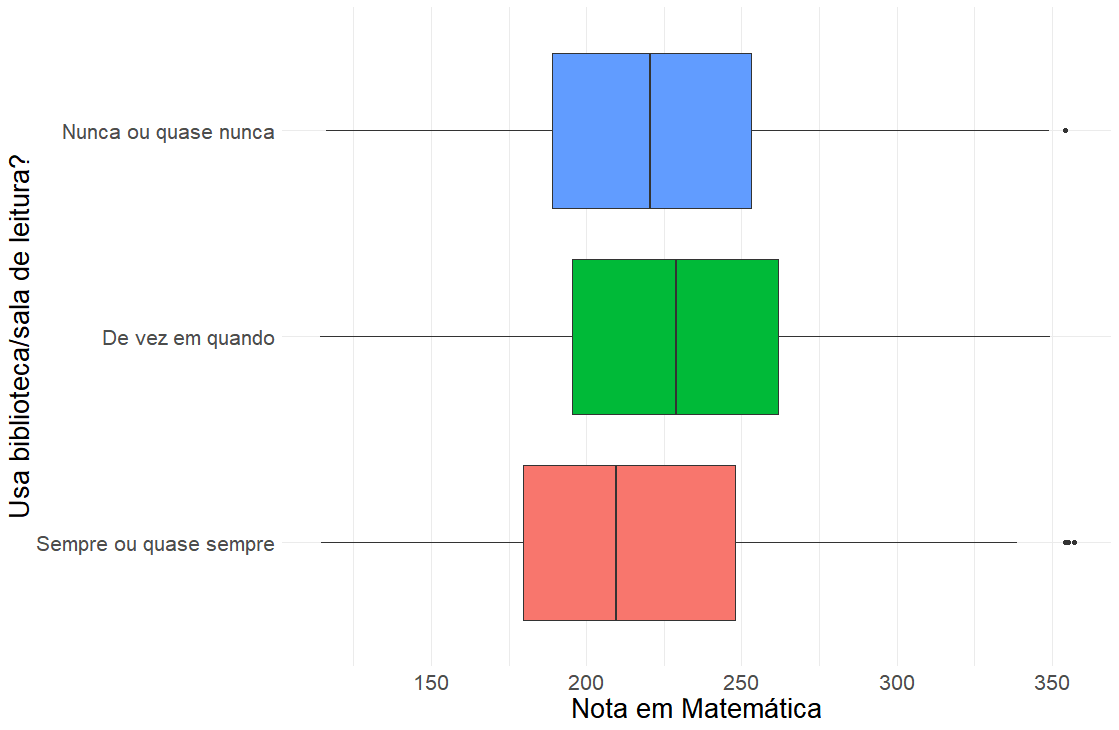
\includegraphics[height=8.2cm,width=12.7cm]{figuras/boxplot_nota_biblioteca.png}
\vspace{-0.2cm}
\label{fig3}
\\ \footnotemark{Fonte:Inep (Instituto Nacional de Estudos e Pesquisas Educacionais Anísio Teixeira). }
\end{figure}

Em relação ao tempo de uso de telas, verificamos a distribuição segundo sexo. Percebemos que há uma inversão na frequência entre meninos e meninas a medidas que são relatadas mais horas em frente às telas. Dessa forma, mais meninas dizem passar até 1 hora, enquanto mais meninos dizem passar mais de 1 hora em frente à TV, computador ou \textit{videogame}. 

\begin{figure}[!ht]
\vspace{-0.25cm}
\caption{Tempo de uso de telas segundo Sexo - SAEB, 2017}
\centering
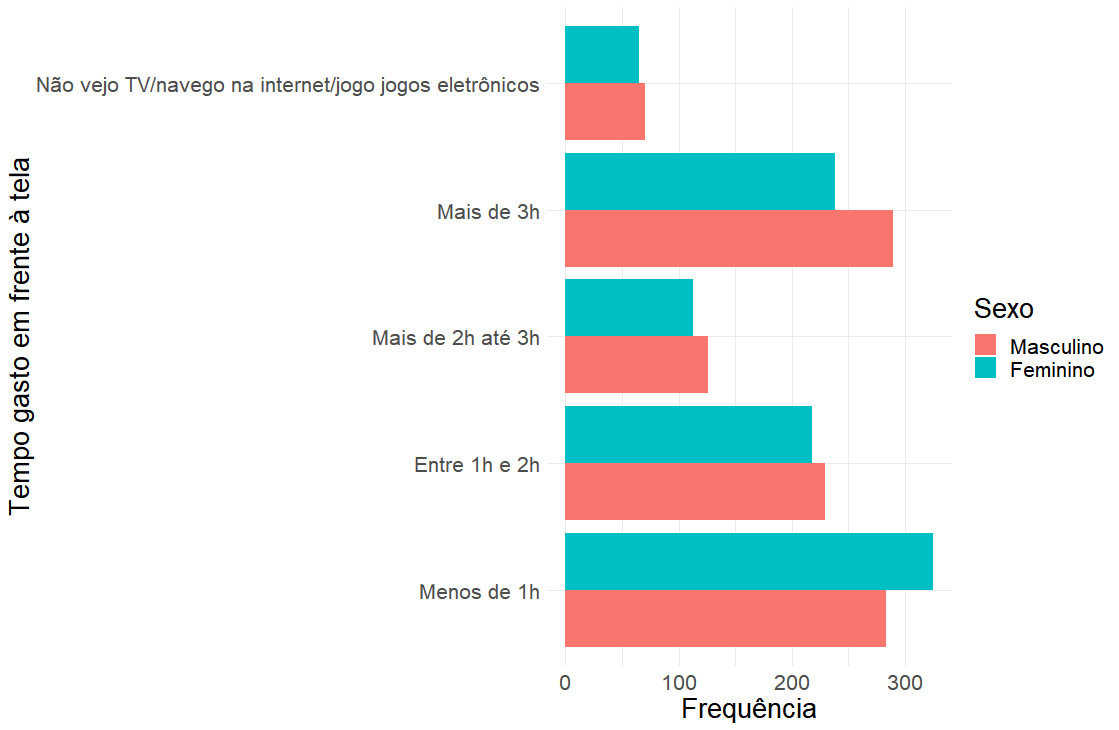
\includegraphics[height=8.2cm,width=12.7cm]{figuras/plot_usotelas_sexo.png}
\vspace{-0.2cm}
\label{fig4}
\\ \footnotemark{Fonte:Inep (Instituto Nacional de Estudos e Pesquisas Educacionais Anísio Teixeira). }
\end{figure}

O tempo de uso também é diferenciado a depender da quantidade de computadores a que os alunos tem acesso. Aqueles que declararam não ter computador tem maior frequência entre os que não navegam ou navegam até 1 hora. A categoria de maior destaque é a dos alunos que possuem 1 computador, com a maior frequência entre os que declaram passar entre 1 e 3 horas em frente às telas.

\begin{figure}[!ht]
\vspace{-0.25cm}
\caption{Tempo de uso de telas segundo acesso à computador - SAEB, 2017}
\centering
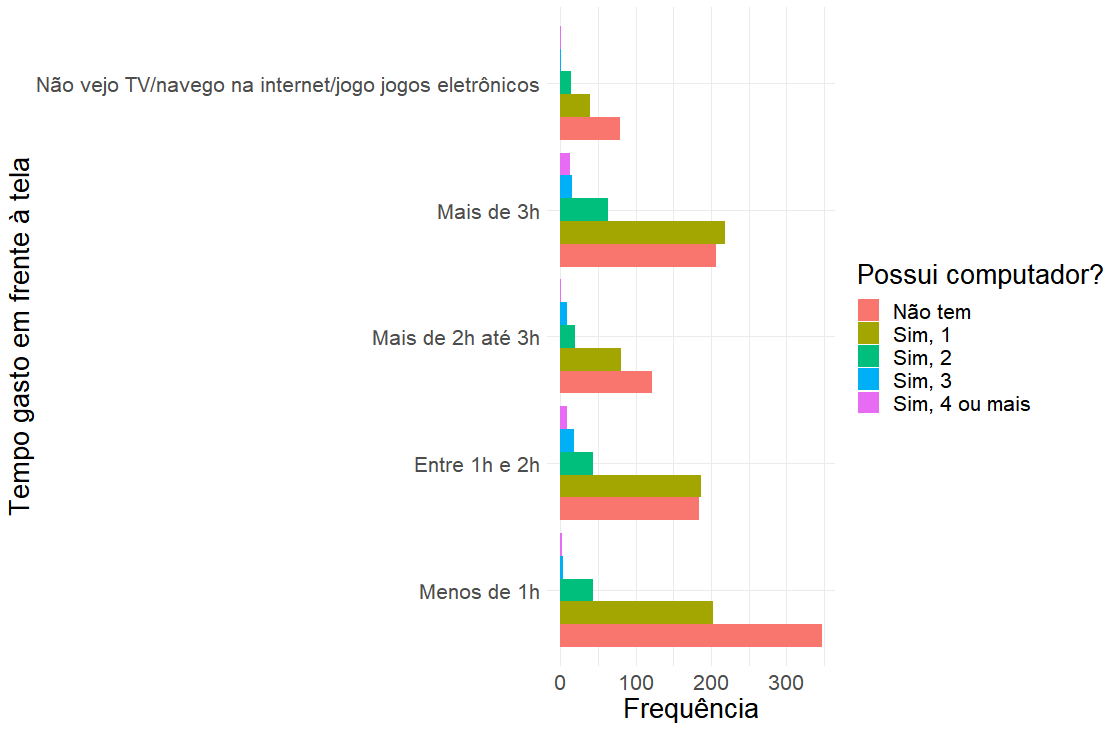
\includegraphics[height=8.2cm,width=12.7cm]{figuras/plot_usotelas_computador.png}
\vspace{-0.2cm}
\label{fig5}
\\ \footnotemark{Fonte:Inep (Instituto Nacional de Estudos e Pesquisas Educacionais Anísio Teixeira). }
\end{figure}

\newpage
\section{Conclusões}
A desigualdade educacional no Brasil é um tema de estudo relevante no cenário sócio-político brasileiro, uma vez que recorrentemente se discutem como possíveis melhorias podem ser aplicadas. Sob a perspectiva da disciplina de Matemática, comumente observamos discrepâncias tanto no ensino quanto no interesse dos alunos. 

Nesse estudo, concluímos que existe diferença de notas significativa das notas em Matemática com relação às variáveis de estudo proporstas -- Área de localização da escola e frequência à biblioteca/sala de estudos. É interessante observar que a região onde a escola está trata-se de um fator externo, enquanto a ida à biblioteca é um fator individual. Ainda assim, ambos tem relevância nas notas dos alunos.

Além disso, também observamos que o tempo gasto com dispositivos eletrônicos tem influência tanto do acesso ao computador quanto do sexo do aluno, ficando claro que alunos do sexo masculino passam mais horas em frente às telas, bem como os alunos que tem pelo menos um computador a que possam acessar.

Desta forma, estudos como esse possuem relevância para avaliar a estrutura e a dimensão do problema de desigualdades em âmbito escolar, pois é possível visualizar quais os pontos de atenção e possíveis melhorias que podem ser propostos, tanto a nível de unidades escolares quanto em nível de estrutura geral escolar. Esse fomento é essencial para futuras políticas públicas mais efetivas e eficazes, tendo em vista mitigar os problemas globais da educação brasileira e potencializar os resultados individuais dos alunos.

Esse é um estudo exploratório e inferencial. No entanto, outros estudos mais aprofundados sobre o assunto são necessários, afim de analisar de forma mais profunda essas relações, propor modelagens e avaliar as correlações entre variáveis explicativas.


\section{Referências}

[1] Blog Estar Saúde Mental. Procrastinação atinge até 90\% da população em geral.
https://www.estarsaudemental.com.br/procrastinacao-atinge-ate-90-da-populacaoem-geral/: :text=A\%20procrastina\%C3\%A7\%C3\%A3o\%20afeta\%20cronicamente\%20de,v\%C3\%A1rias\%20explica\%C3\%A\%C3

\%B5es\%20para\%20a\%20procrastina\%C3\%A7\%C3\%A3o, 2017.


[2] Vanessa Castro de Oliveira, Cristiano Peres Oliveira, and Francieli Aparecida Vaz. A história da matemática e o processo de ensino aprendizagem. 2014.

\end{document}